\chapter{Desenvolvimento do Trabalho}
\label{c.desenvolvimento}

\section{Modelo de Pesquisa}
\label{s.metodo}

A Figura ~\ref{f.metodopesquisa} apresenta um diagrama com os principais elementos deste projeto de pesquisa. As elipses representam temas ou assuntos. Os retângulos com cantos arredondados, atividades. As setas representam as relações entre diferentes elementos. Os cilindros representam bases de dados de artigos científicos.

\begin{figure}[H]
	\caption{\small Modelo de Pesquisa.}
	\centering
	\includegraphics[scale=0.7]{Imagens/metodologia.png}
	\label{f.metodopesquisa}
	\legend{\small Fonte: Elaborada pelo autor.}
\end{figure}

A pesquisa foi dividida em seis etapas. A princípio (fundamentação teórica) foi feito um levantamento bibliográfico sobre os tipos de controle físicos que podem ser utilizados no celular, ferramentas para o desenvolvimento de aplicações em realidade virtual e métodos de avaliação para controles físicos.

A segunda etapa (preparação do ambiente operacional), envolveu a escolha dos \textit{software} a serem utilizados com base na exequibilidade do projeto e da acessibilidade das ferramentas, ou seja, foram capazes de proporcionar as vias necessárias para o êxito do projeto de forma gratuita e com documentação clara. 

Na terceira fase do projeto (escolha dos controles físicos), foi feita a escolha de três tipos de controles que apresentam três diferentes tipos de conexão e interatividade: via cabo, \textit{Bluetooth} e toque na tela. 

Na quarta etapa (desenvolvimento da aplicação em RV), foi realizada a construção da aplicação, juntamente com os testes e correções considerando a usabilidade da mesma.

A quinta etapa (análise dos controles), verificou se o projeto atingiu os objetivos geral e específicos propostos levando em consideração a análise dos controles em relação as suas características de usabilidade, experiência e funcionalidade. 

Na última (sexta) etapa (relatório de pesquisa), foi elaborado o relatório final da pesquisa registrando todos os procedimentos realizados bem como os resultados e conclusões.

\section{Controles}

\subsection{Controle Google Cardboard 2.0}
\label{ss.cardboard}

Como mencionado anteriormente, o Google Cardboard 2.0 utiliza o toque na tela como forma de interação. Apesar de ser totalmente feito em papelão, este visualizador é montado de forma que ao pressionar um botão na parte superior do mesmo, o toque na tela é realizado. Como \textit{smartphones} não reconhecem o contato do papelão na tela, a parte que realiza o contato é revestido por tecido condutivo.

\subsection{Controle via Cabo}
\label{ss.cabo}

Para a conexão via cabo, é necessário somente um cabo \textit{On-The-Go} (OTG) (Figura ~\ref{f.otg}) e um controle de vídeo game que possua interface USB. O USB OTG foi criado em 2001 e seu objetivo é aumentar a capacidade de dispositivos móveis adicionando funcionalidade de \textit{host} para conexões de periféricos com conexão USB. A ideia é a de, ao conectar um periférico ao cabo OTG, o mesmo funcione automaticamente sem a necessidade de configurações adicionais. \cite{otg}
Exemplos de dispositivos compatíveis são controles da Playstation® e Xbox®. No caso dos controles mais antigos da Playstation® que não possuem cabos USB, é possível adquirir um adaptador como o da Figura ~\ref{f.adaptador}.

\begin{figure}[H]
	
	\begin{minipage}{.5\textwidth}{
			\centering
			\captionof{figure}{\small Cabo USB OTG}
			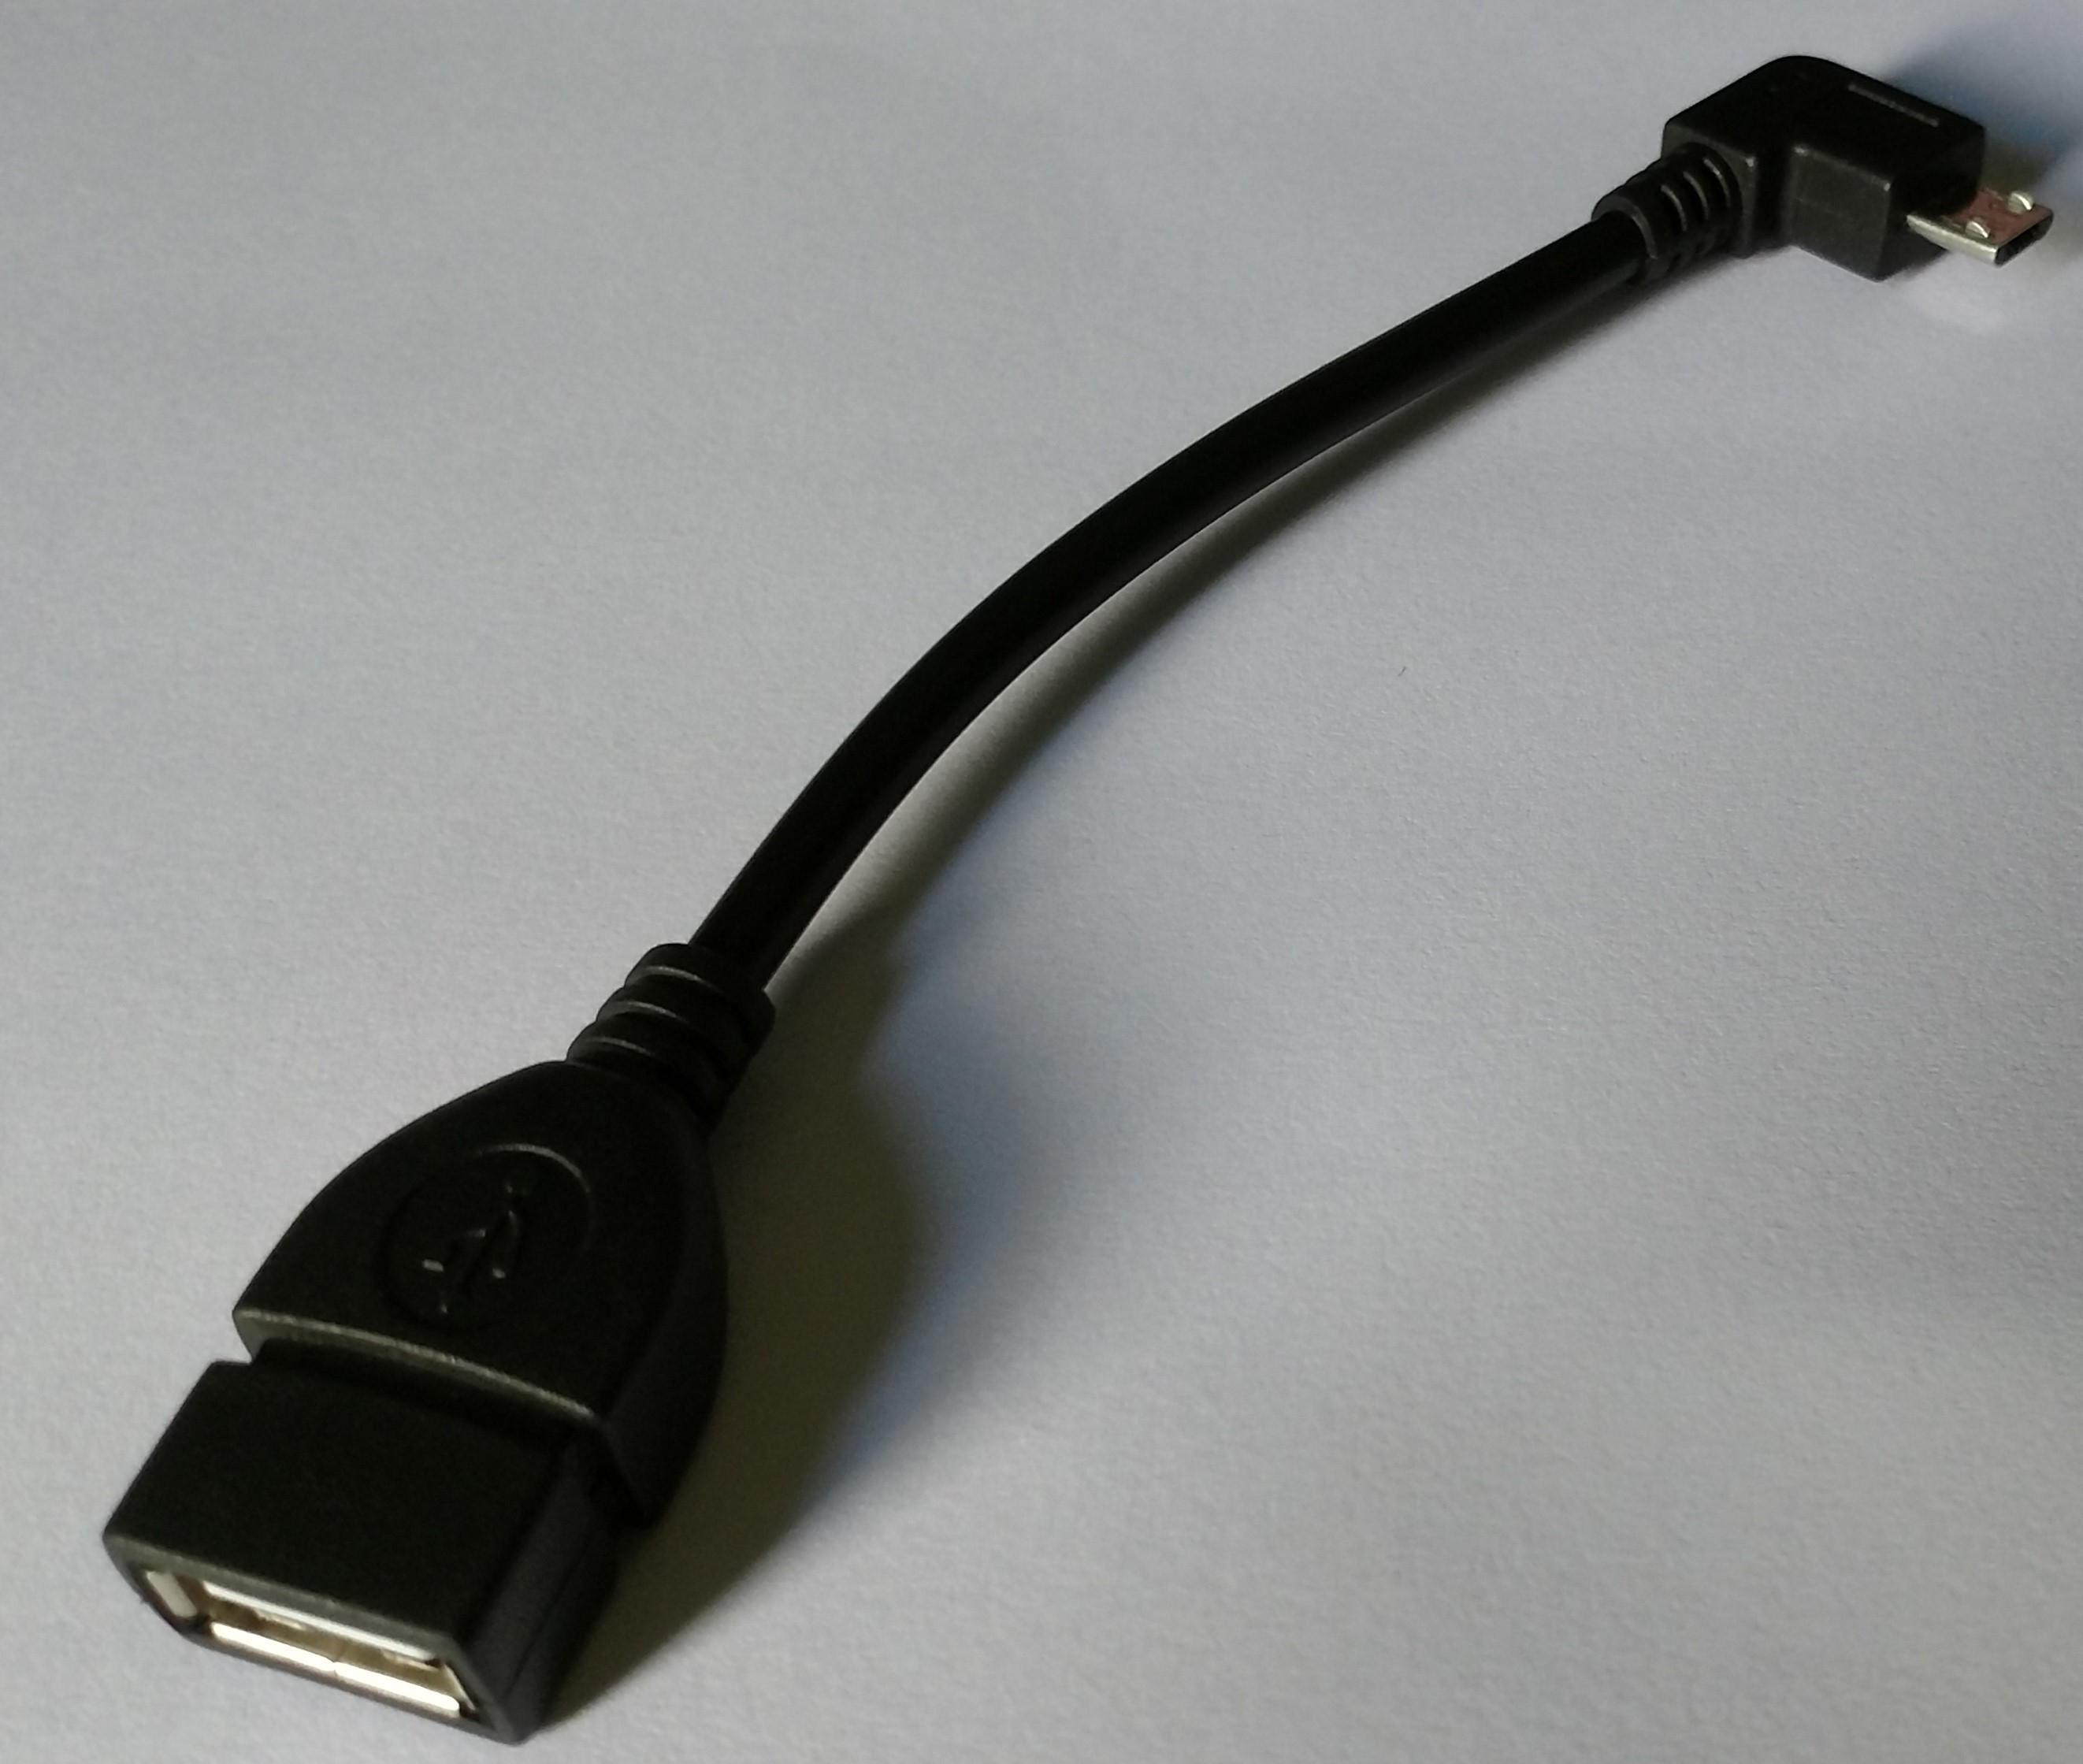
\includegraphics[height=4cm]{Imagens/otg.jpg}		
			\label{f.otg}	
			\legend{\small Fonte: Elaborada pelo autor.}
		}
	\end{minipage}
	\begin{minipage}{.5\textwidth}{
			\centering
			\captionof{figure}{\small Adaptador USB}
			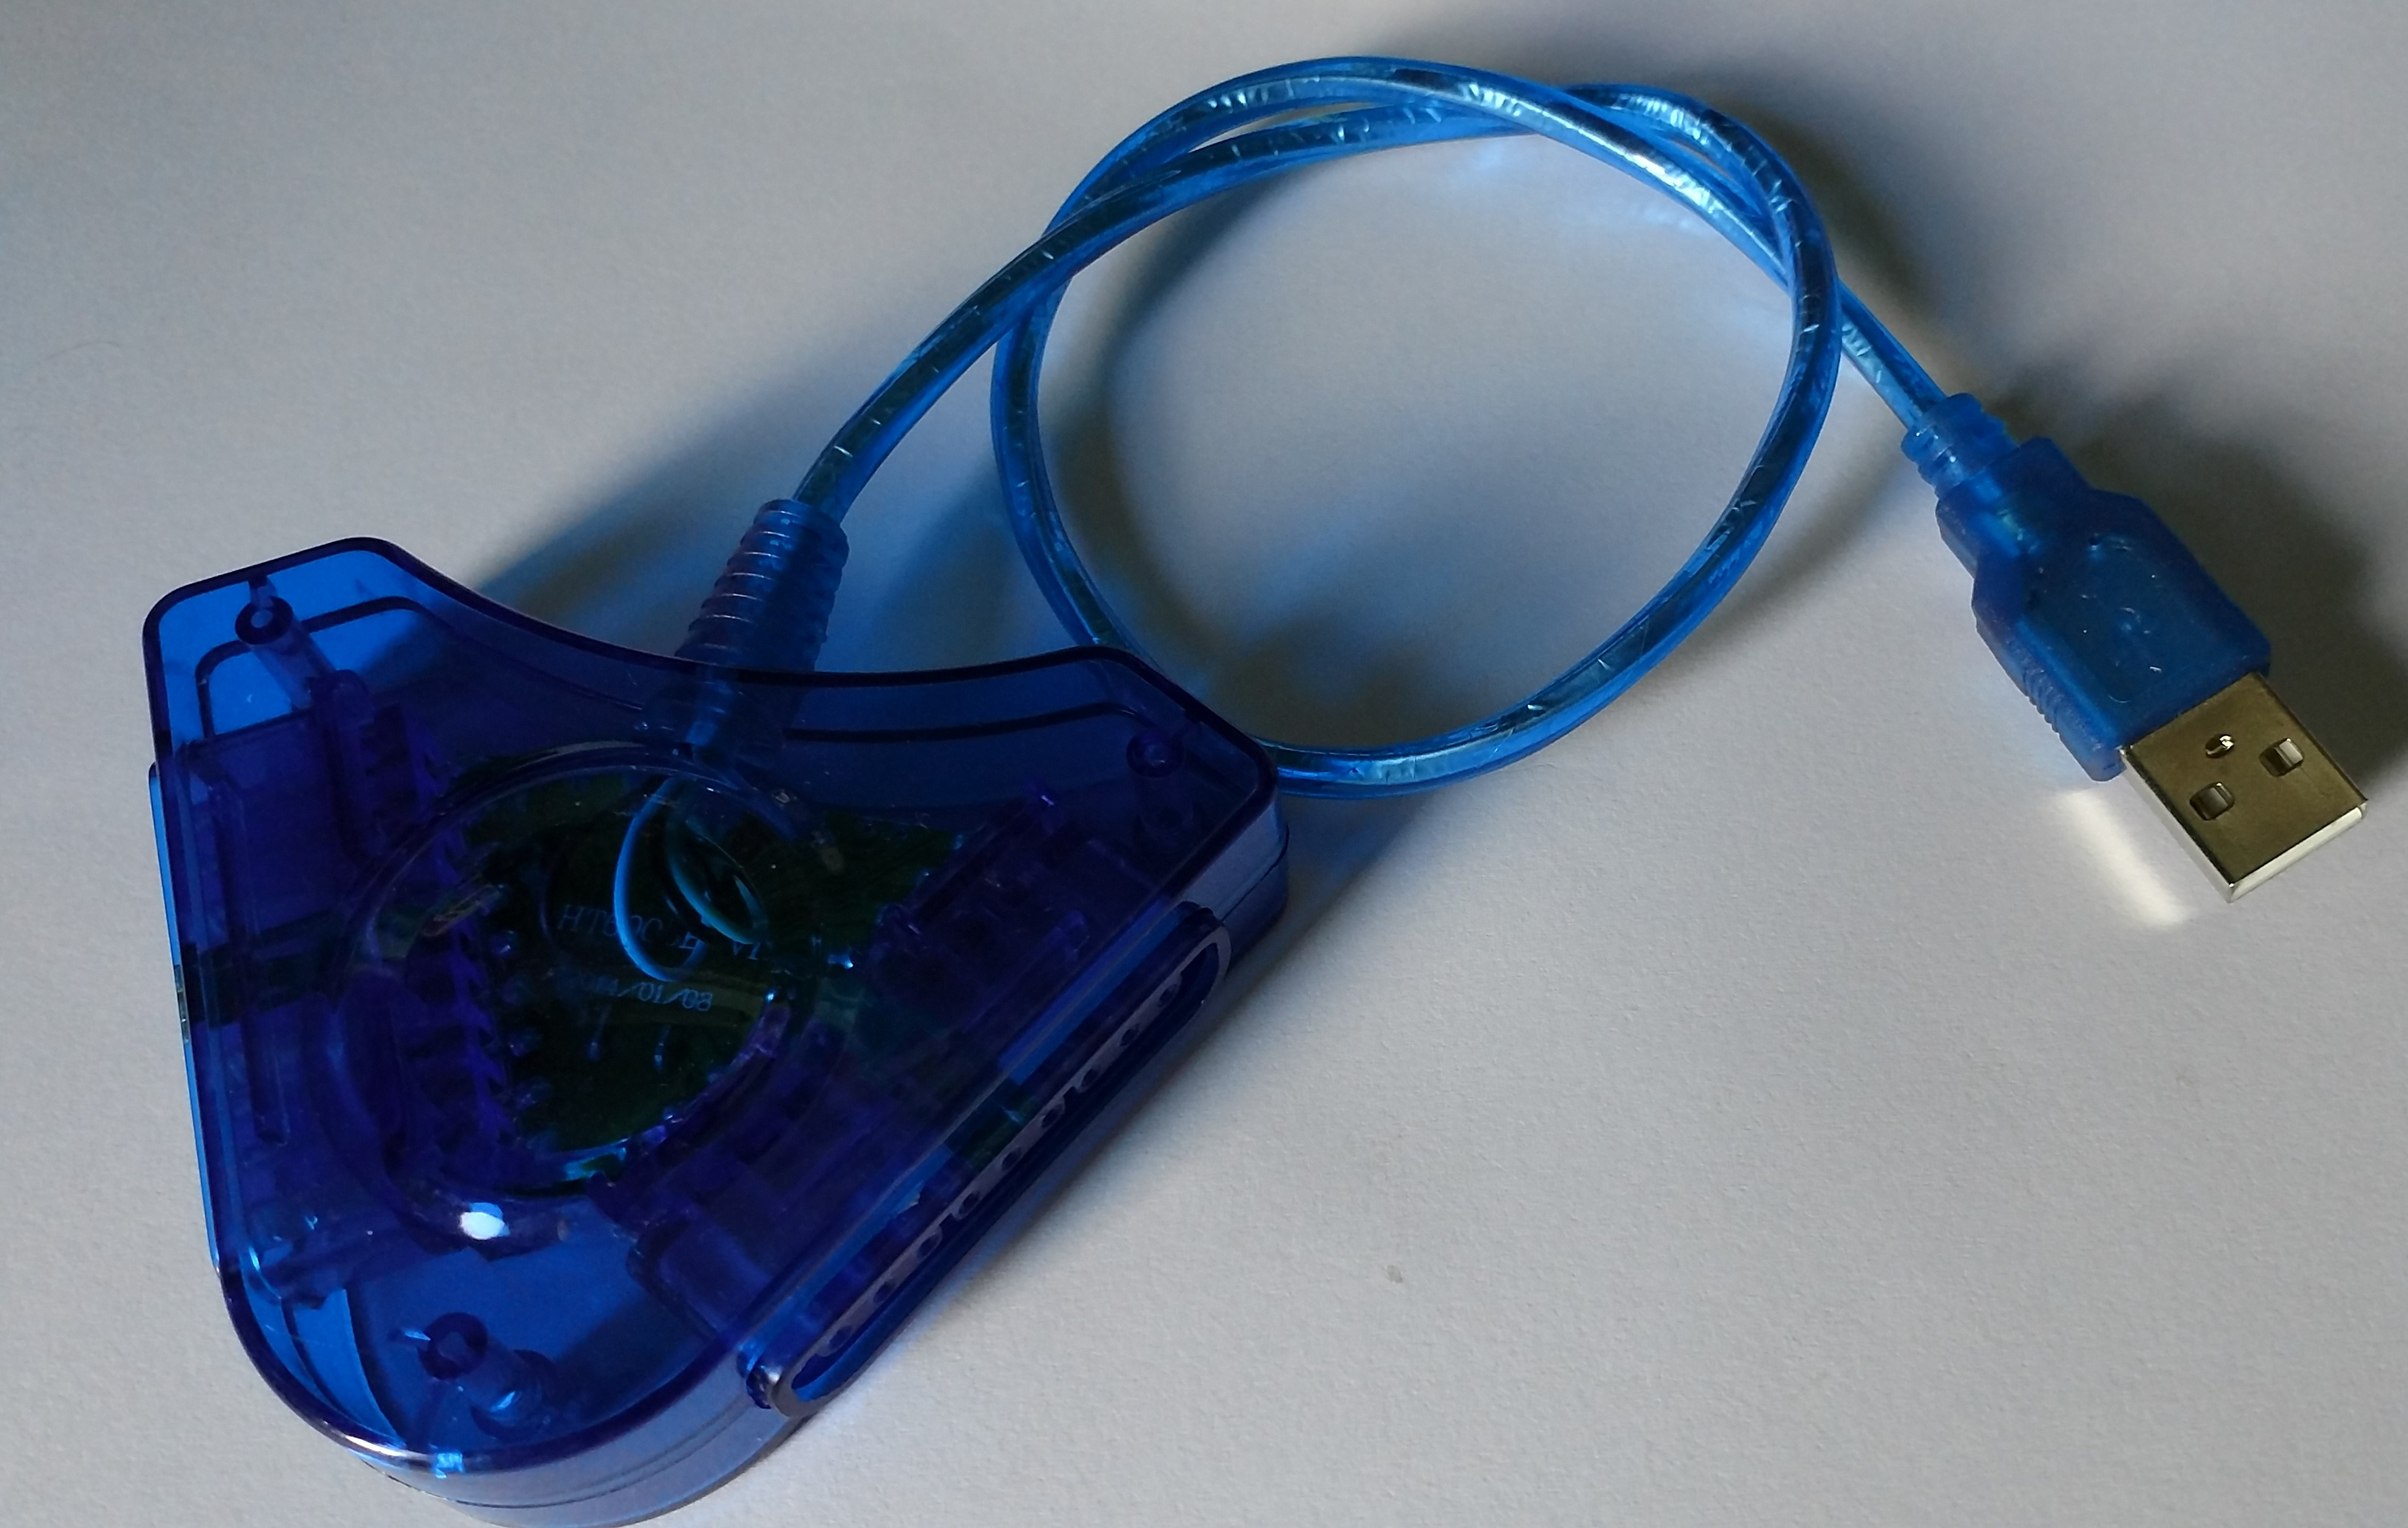
\includegraphics[height=4cm]{Imagens/adaptador.jpg}		
			\label{f.adaptador}
			\legend{\small Fonte: Elaborada pelo autor.}	
		}
	\end{minipage}
	
\end{figure}

\subsection{Controle Bluetooth}

A tecnologia \textit{Bluetooth} está presente em diversos dispositivos ao redor do mundo, inclusive nos telefones celulares. Pode ser utilizada como forma de comunicação entre \textit{smartphones} e periféricos.

\begin{citacao}
	"Um dispositivo \textit{Bluetooth} utiliza ondas de rádio ao invés de cabos para se conectar a um celular ou computador. Um produto \textit{Bluetooth} como um fone de ouvido ou relógio, possui um pequeno chip de computador com rádio \textit{Bluetooth} e software que facilita a conexão. Quando dois dispositivos \textit{Bluetooth} querem trocar informações, eles precisam ser pareados." \cite[tradução nossa]{bluetooth}
\end{citacao}

Para este projeto, foram explorados dois dispositivos \textit{Bluetooth} que podem ser utilizados como dispositivos de controle do usuário com a aplicação em realidade virtual. O primeiro consiste em um teclado de computador que utiliza o \textit{Bluetooth} como forma de comunicação. Atualmente é possível encontrar este tipo de teclado que, além de se comunicar com o computador, também se conecta com dispositivos móveis sem que seja necessário a instalação de softwares específicos. 

O outro dispositivo utilizado foi um \textit{joystick} que utiliza a comunicação \textit{Bluetooth}. Atualmente encontra-se no mercado alguns controles com esta característica como o \textit{Wii Remote}, controle que acompanha o console Nintendo Wii® (Figura ~\ref{f.wiiremote}), e o controle da VR Box (Figura ~\ref{f.controlevrbox}) que acompanha o capacete de visualização da mesma empresa.

\begin{figure}[H]
	
	\begin{minipage}{.5\textwidth}{
			\centering
			\captionof{figure}{\small Wii Remote}
			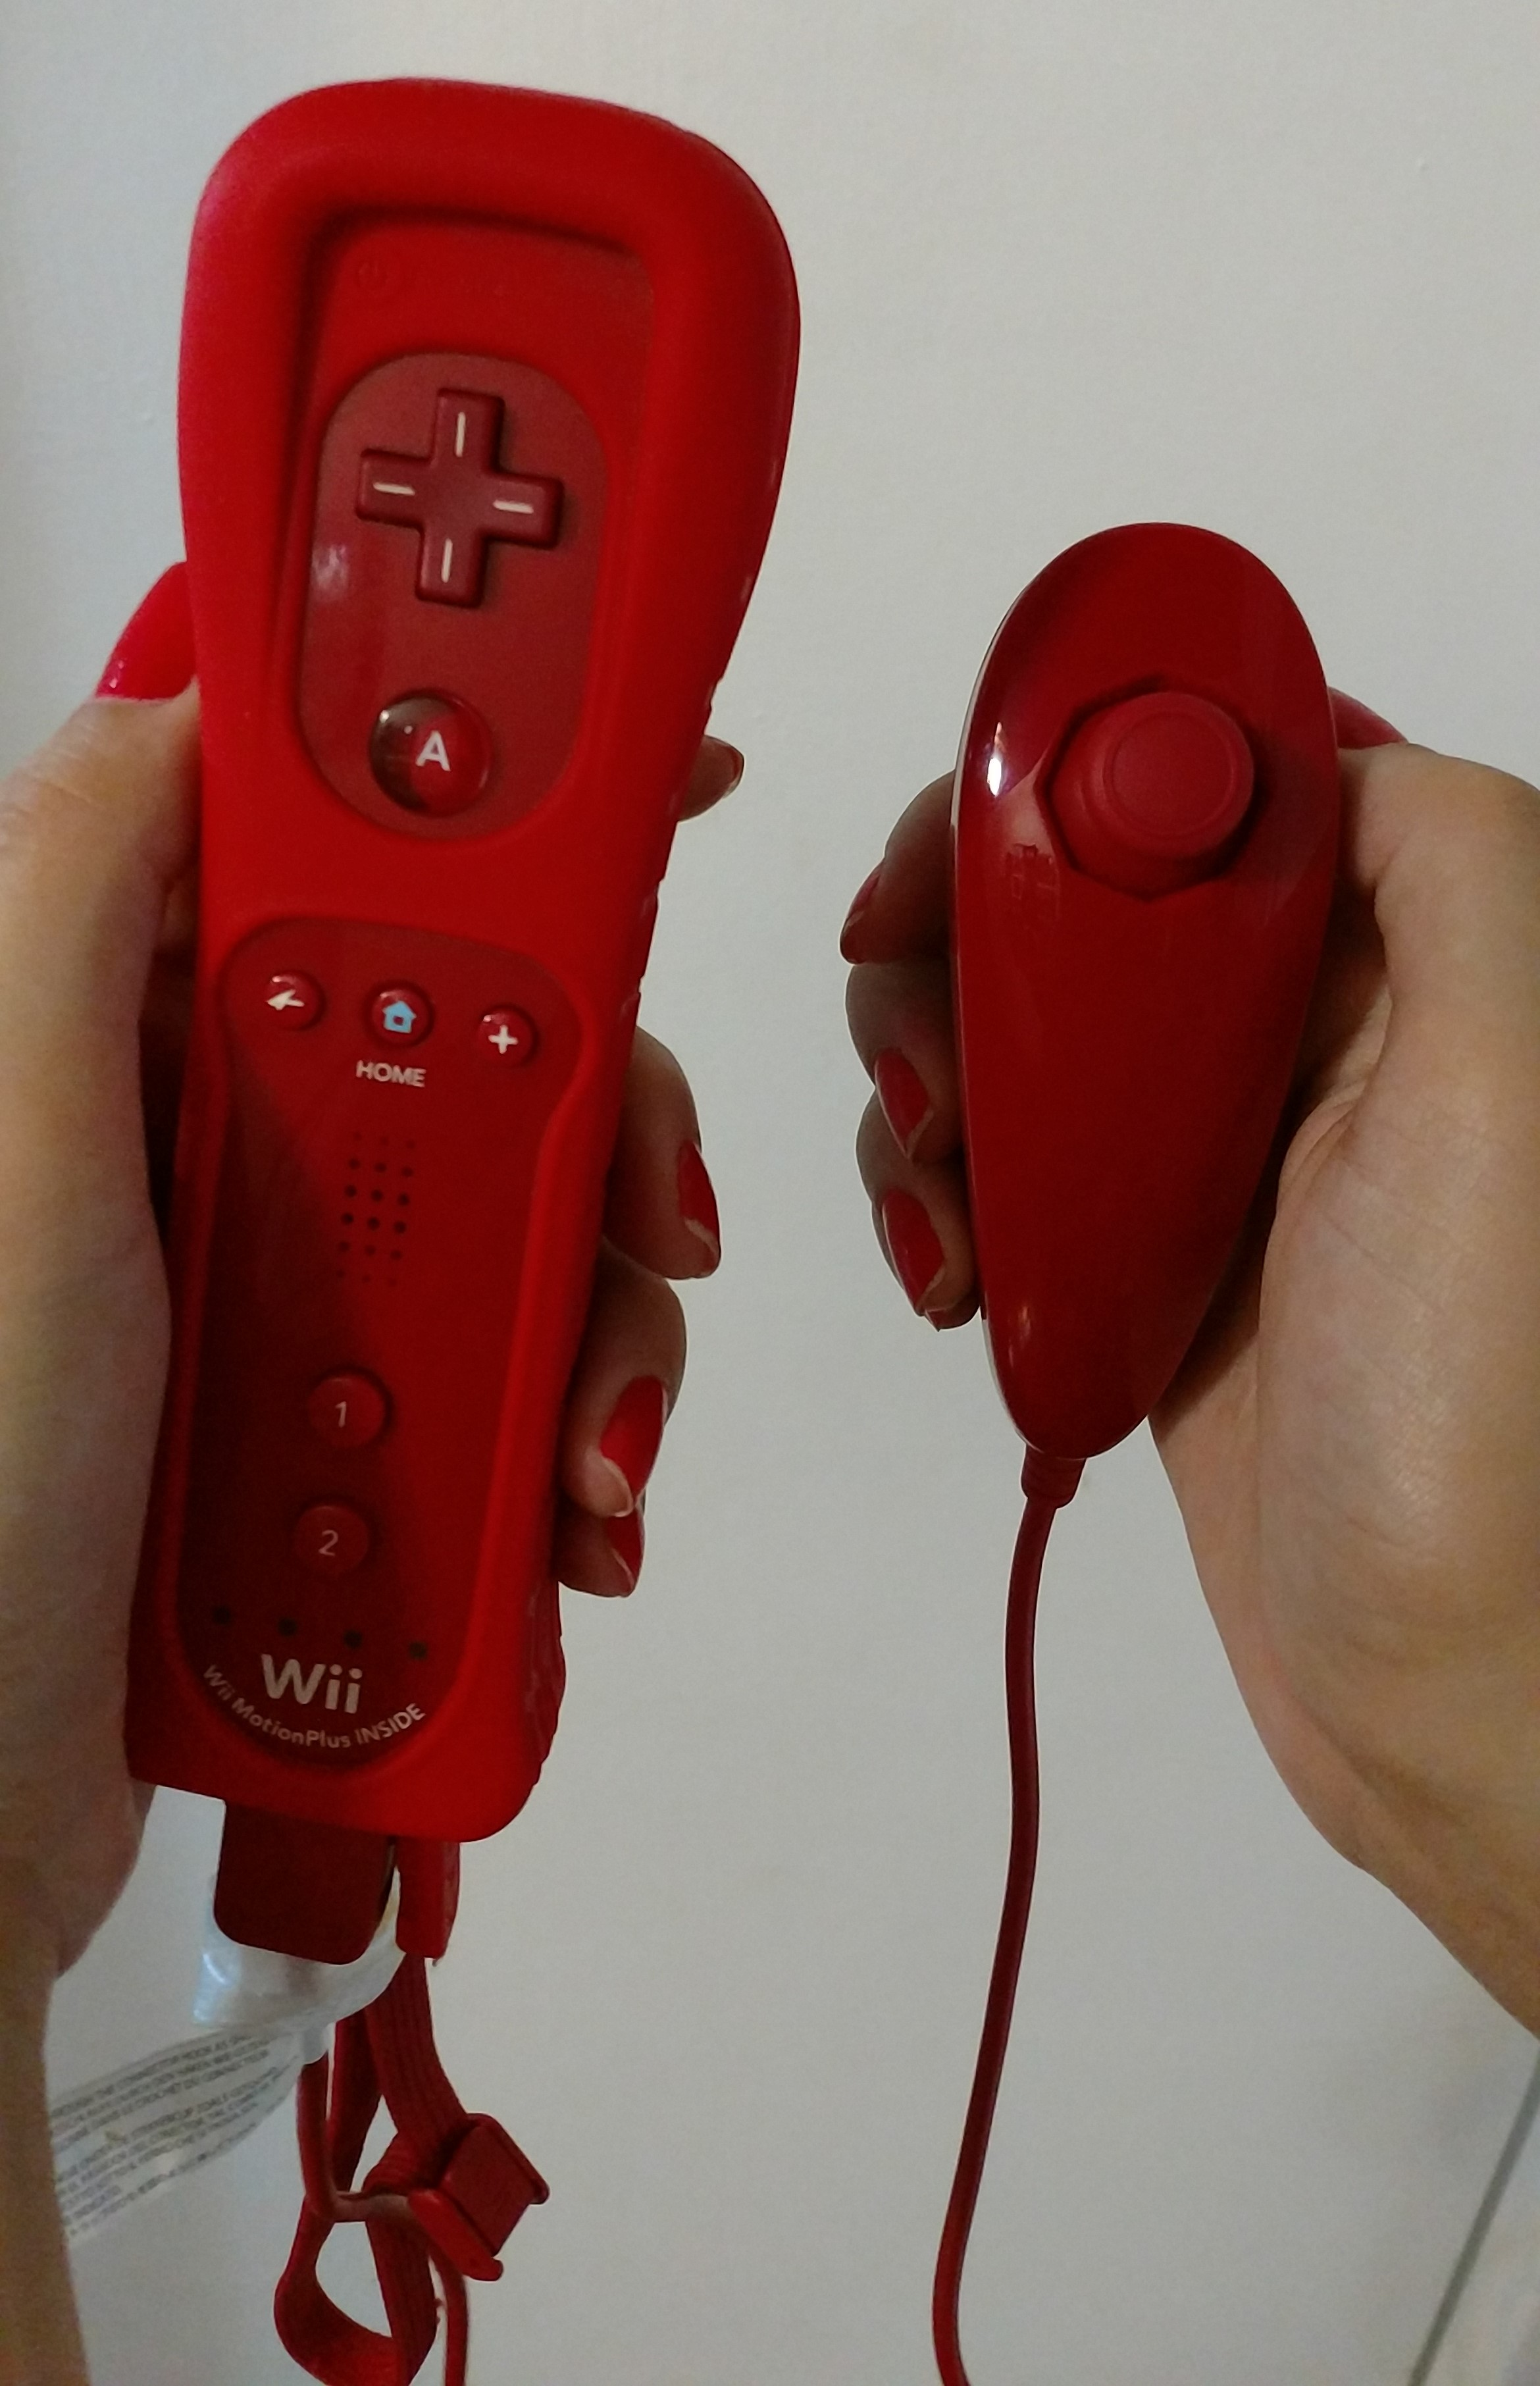
\includegraphics[width=.7\linewidth]{Imagens/wiiremote.jpg}		
			\label{f.wiiremote}	
			\legend{\small Fonte: Elaborada pelo autor.}
		}
	\end{minipage}
	\begin{minipage}{.5\textwidth}{
			\centering
			\captionof{figure}{Controle VR Box}
			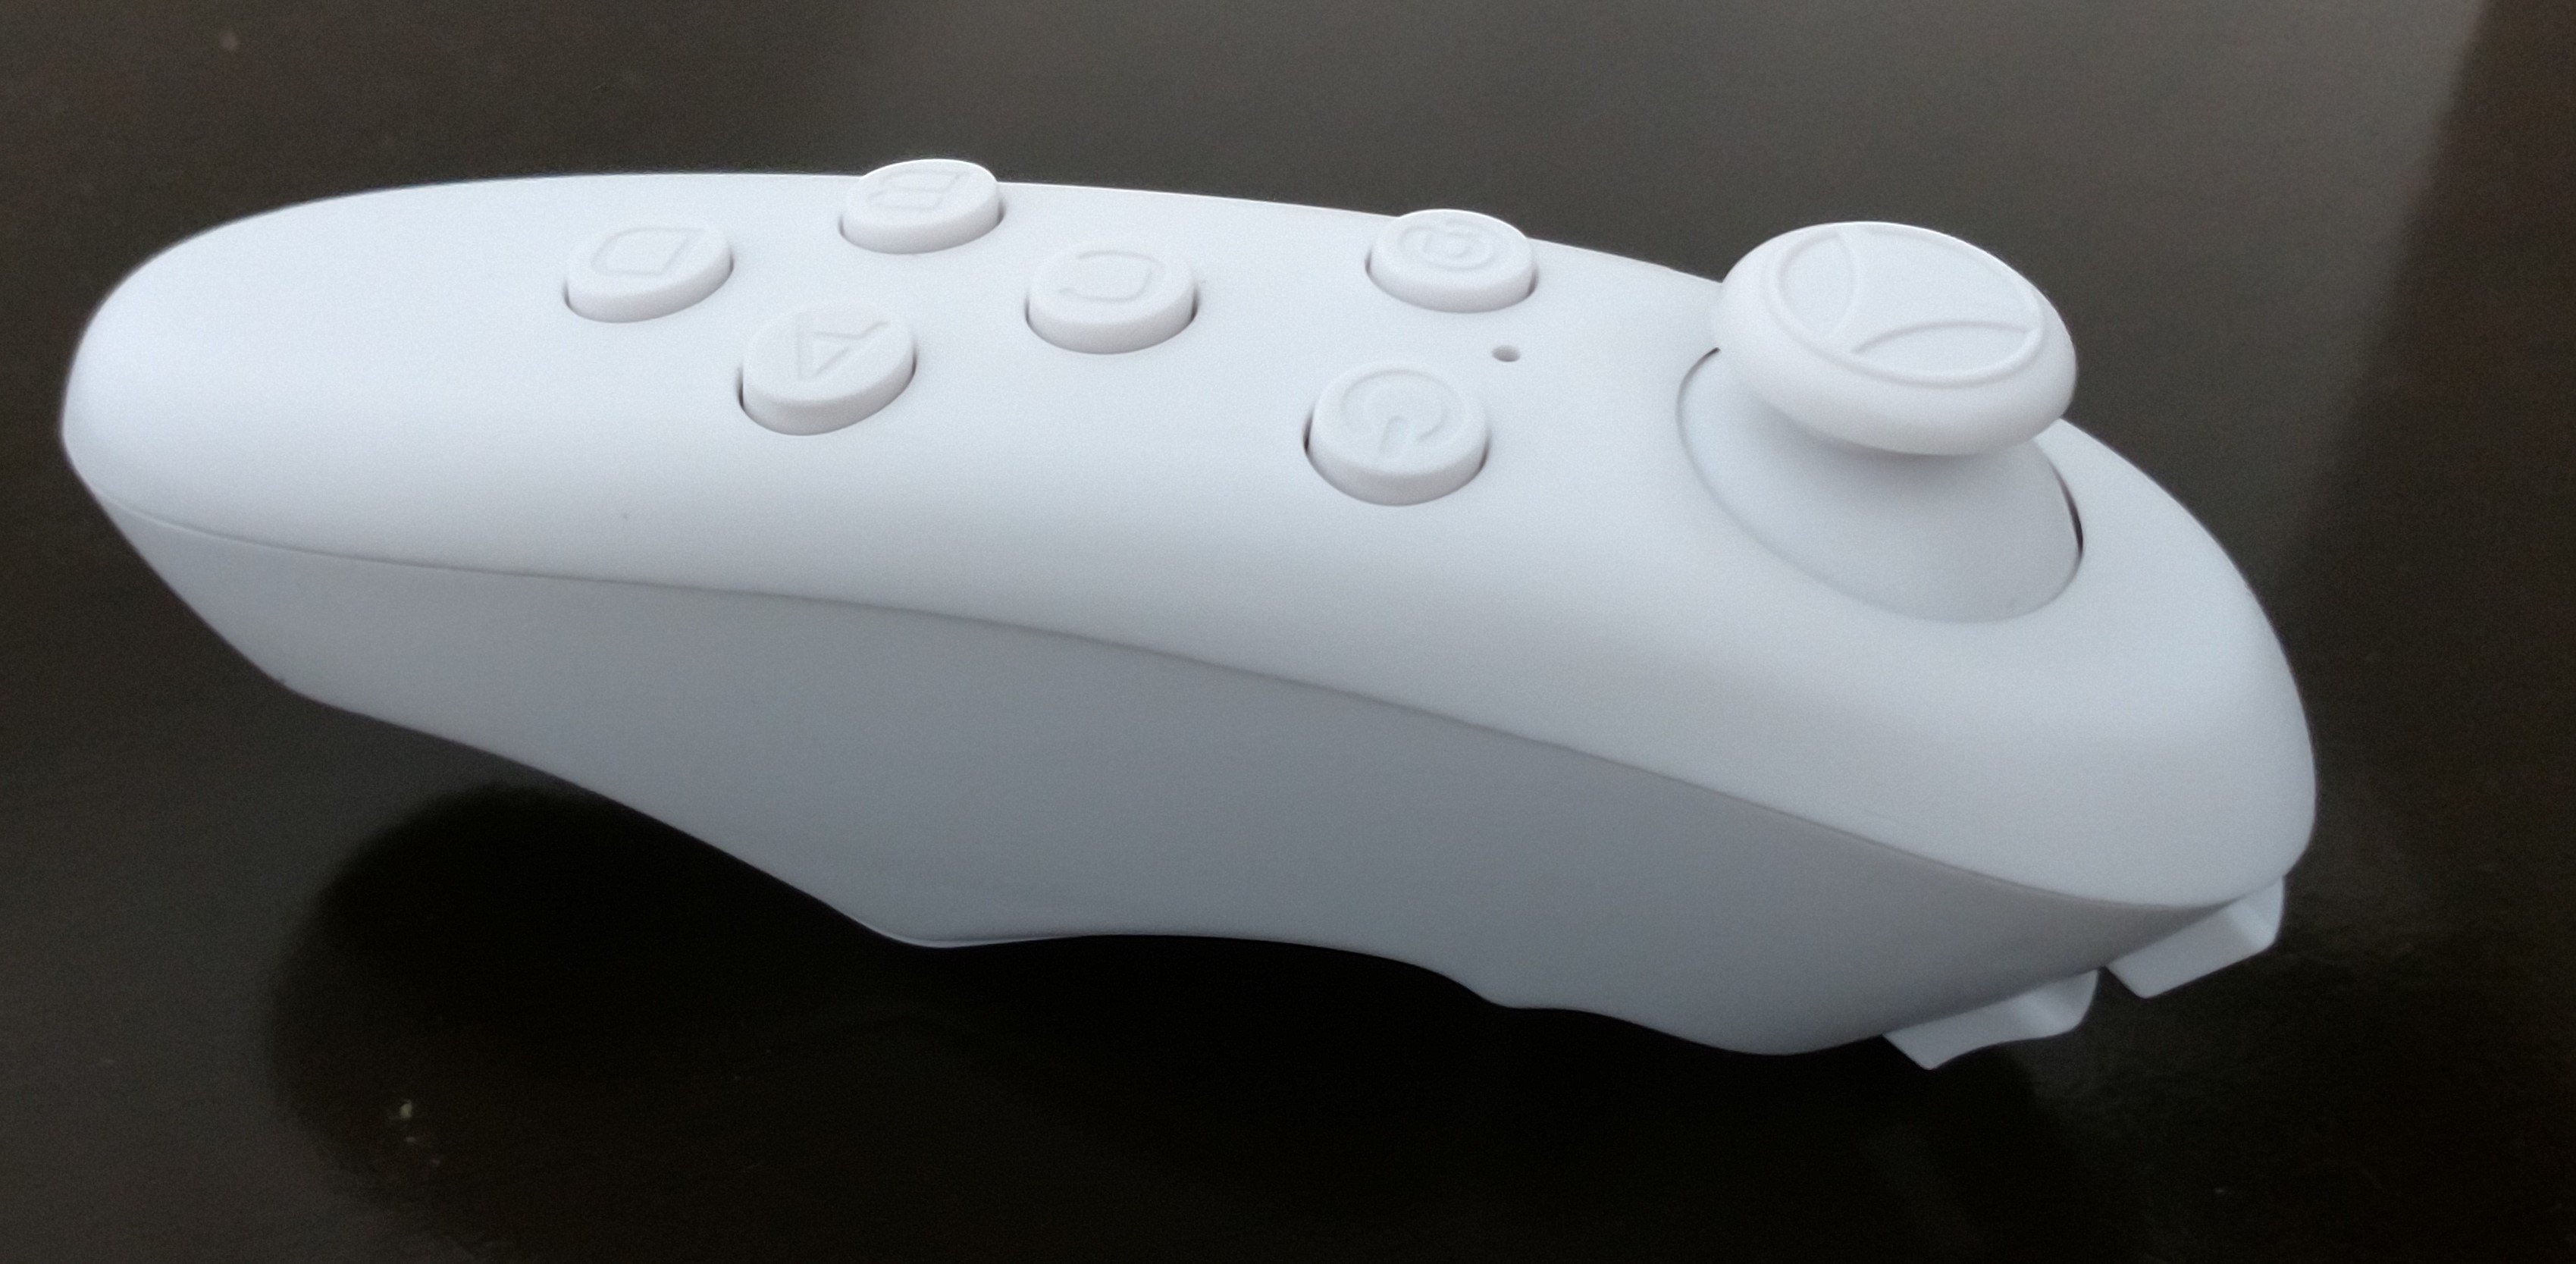
\includegraphics[width=.7\linewidth]{Imagens/controlevrbox.jpg}		
			\label{f.controlevrbox}
			\legend{\small Fonte: Elaborada pelo autor.}	
		}
	\end{minipage}
	
\end{figure}

Para este projeto, o \textit{joystick} utilizado foi o fornecido pela empresa VR Box pois o mesmo permite a conexão com dispositivos móveis diferentemente do \textit{Wii Remote} que não possui suporte para este tipo de conexão.

\section{Ferramentas de Desenvolvimento}
\label{s.ferramentas}

\subsection{Unity}
\label{ss.unity}
Tendo em vista que a aplicação foi feita em um dispositivo com sistema operacional Android, a ferramenta de desenvolvimento escolhida deve oferecer suporte para este tipo de dispositivo. A Google® oferece um conjunto de ferramentas denominado \textit{System Development Kit} (SDK) para desenvolvimento em RV. Os SDKs oferecidos contém todo o material necessário para a programação nas seguintes plataformas: Android, Unity, iOS e Unreal Engine 4. \cite{googledocumentacao} 

As opções contam com um projeto exemplo e materiais explicativos sobre o desenvolvimento de aplicações em realidade virtual. Além disso, a Google® oferece guias de boas práticas para a criação de aplicações em RV. 

Após análise, foi escolhido o SDK do Unity para o desenvolvimento da aplicação pois o mesmo oferece um ambiente gráfico intuitivo que não depende somente do código puro. Além disso, o Unity possibilita a exportação da aplicação para múltiplas plataformas (inclusive para dispositivos Android) de forma simples e rápida.

Segundo a empresa \citeonline{unitynumbers}, esta ferramenta é o principal software de desenvolvimento de jogos em escala global com 5 bilhões de jogos feitos em Unity baixados no 3º semestre de 2016 e 770 milhões de pessoas que jogam jogos feitos com a ferramenta. Na área da RV, é estimado que 90\% dos jogos desenvolvidos para o Samsung Gear VR e 53\% dos jogos desenvolvidos para o Oculus Rift foram feitos através do Unity.

O ambiente de desenvolvimento do Unity pode ser visualizado na Figura ~\ref{f.unity}, onde o menu do lado esquerdo contém os objetos presentes na cena, o centro contém a cena em si e o lado direito as propriedades dos objetos selecionados. Esta disposição dos elementos pode ser personalizada pelo usuário. Em cada elemento da cena, é possível adicionar \textit{scripts} que definirão as ações sobre os objetos, podendo ser decorrentes do \textit{input} do usuário e do estado da aplicação em geral. O Unity utiliza duas linguagens de programação para a criação de \textit{scripts}: C\# e UnityScript.  

\begin{figure}[H]
	\caption{\small Unity}
	\centering
	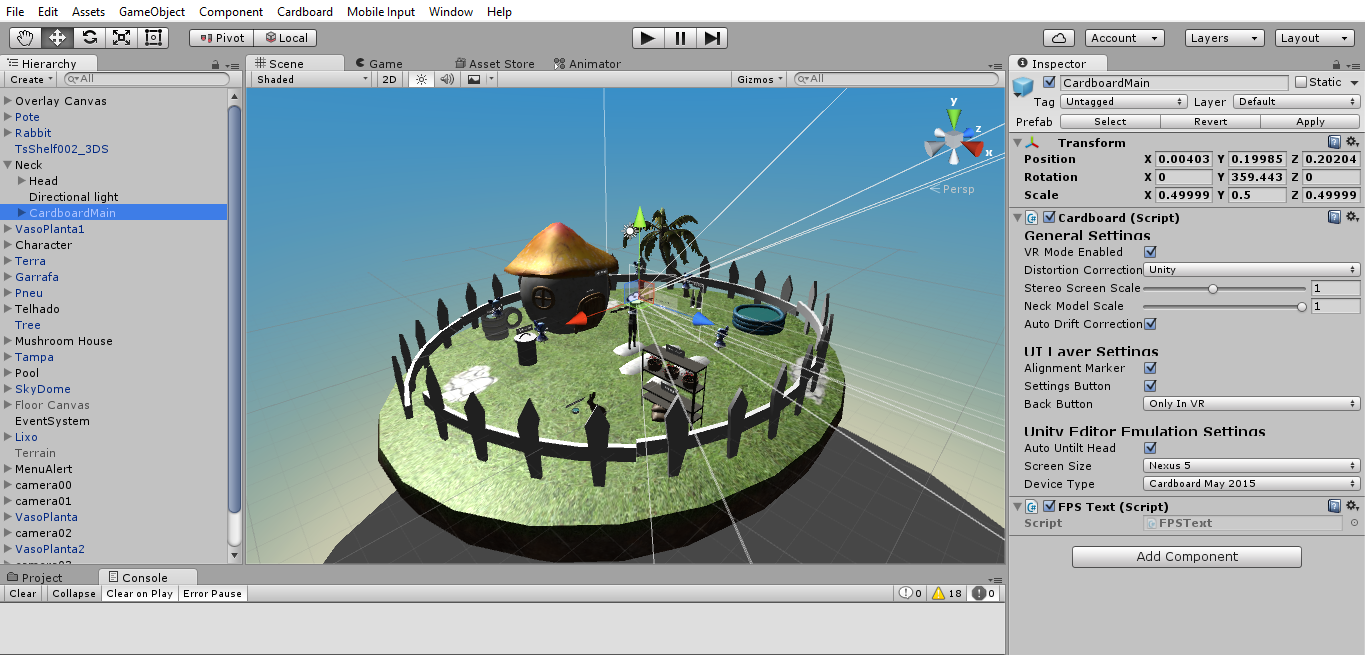
\includegraphics[height=6cm]{Imagens/unity.png}
	\label{f.unity}
	\legend{\small Fonte: Elaborada pelo autor.}
\end{figure}

A fim de criar uma imagem para cada olho e proporcionar a sensação de imersão, são utilizadas duas câmeras (uma para cada olho). De acordo com a documentação oficial do Unity, para mover ou girar a câmera, é preciso anexar as mesmas à um objeto. Desta forma, ao movimentar o objeto, as câmeras refletirão o movimento. 

\subsection{Integração Unity e Google VR}
\label{ss.unitygoogle}

Para facilitar o desenvolvimento de aplicações para o Google Cardboard e o Daydream, o Unity possui integração nativa com o Google VR. Para recursos adicionais, a Google® disponibiliza a Google VR SDK que requer a versão 5.2.1 ou superior do Unity e traz recursos como áudio espacial, suporte para o controle Daydream, ferramentas utilitárias e exemplos.  Segundo a \citeonline{googleunity}, a integração do Unity com o Google VR possibilita a localização da cabeça do usuário, renderização stereo, entre outros. 

\subsection{Capacetes de Visualização}
\label{ss.capacetes}

Para este projeto, foram utilizados dois capacetes de visualização: o Google Cardboard (Figura ~\ref{f.googlecardboard}) e o VR Box (Figura ~\ref{f.vrbox}). Ambos foram escolhidos devido ao baixo custo e por utilizarem um \textit{smartphone} como \textit{display}. 

\begin{figure}[H]
	
	\begin{minipage}{.5\textwidth}{
			\centering
			\captionof{figure}{\small Google Cardboard}
			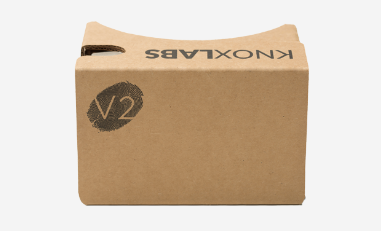
\includegraphics[height=4cm]{Imagens/googlecardboard.png}		
			\label{f.googlecardboard}	
			\legend{\small Fonte: \citeonline{googlecardboard}.}
		}
	\end{minipage}
	\begin{minipage}{.5\textwidth}{
			\centering
			\captionof{figure}{\small VR Box}
			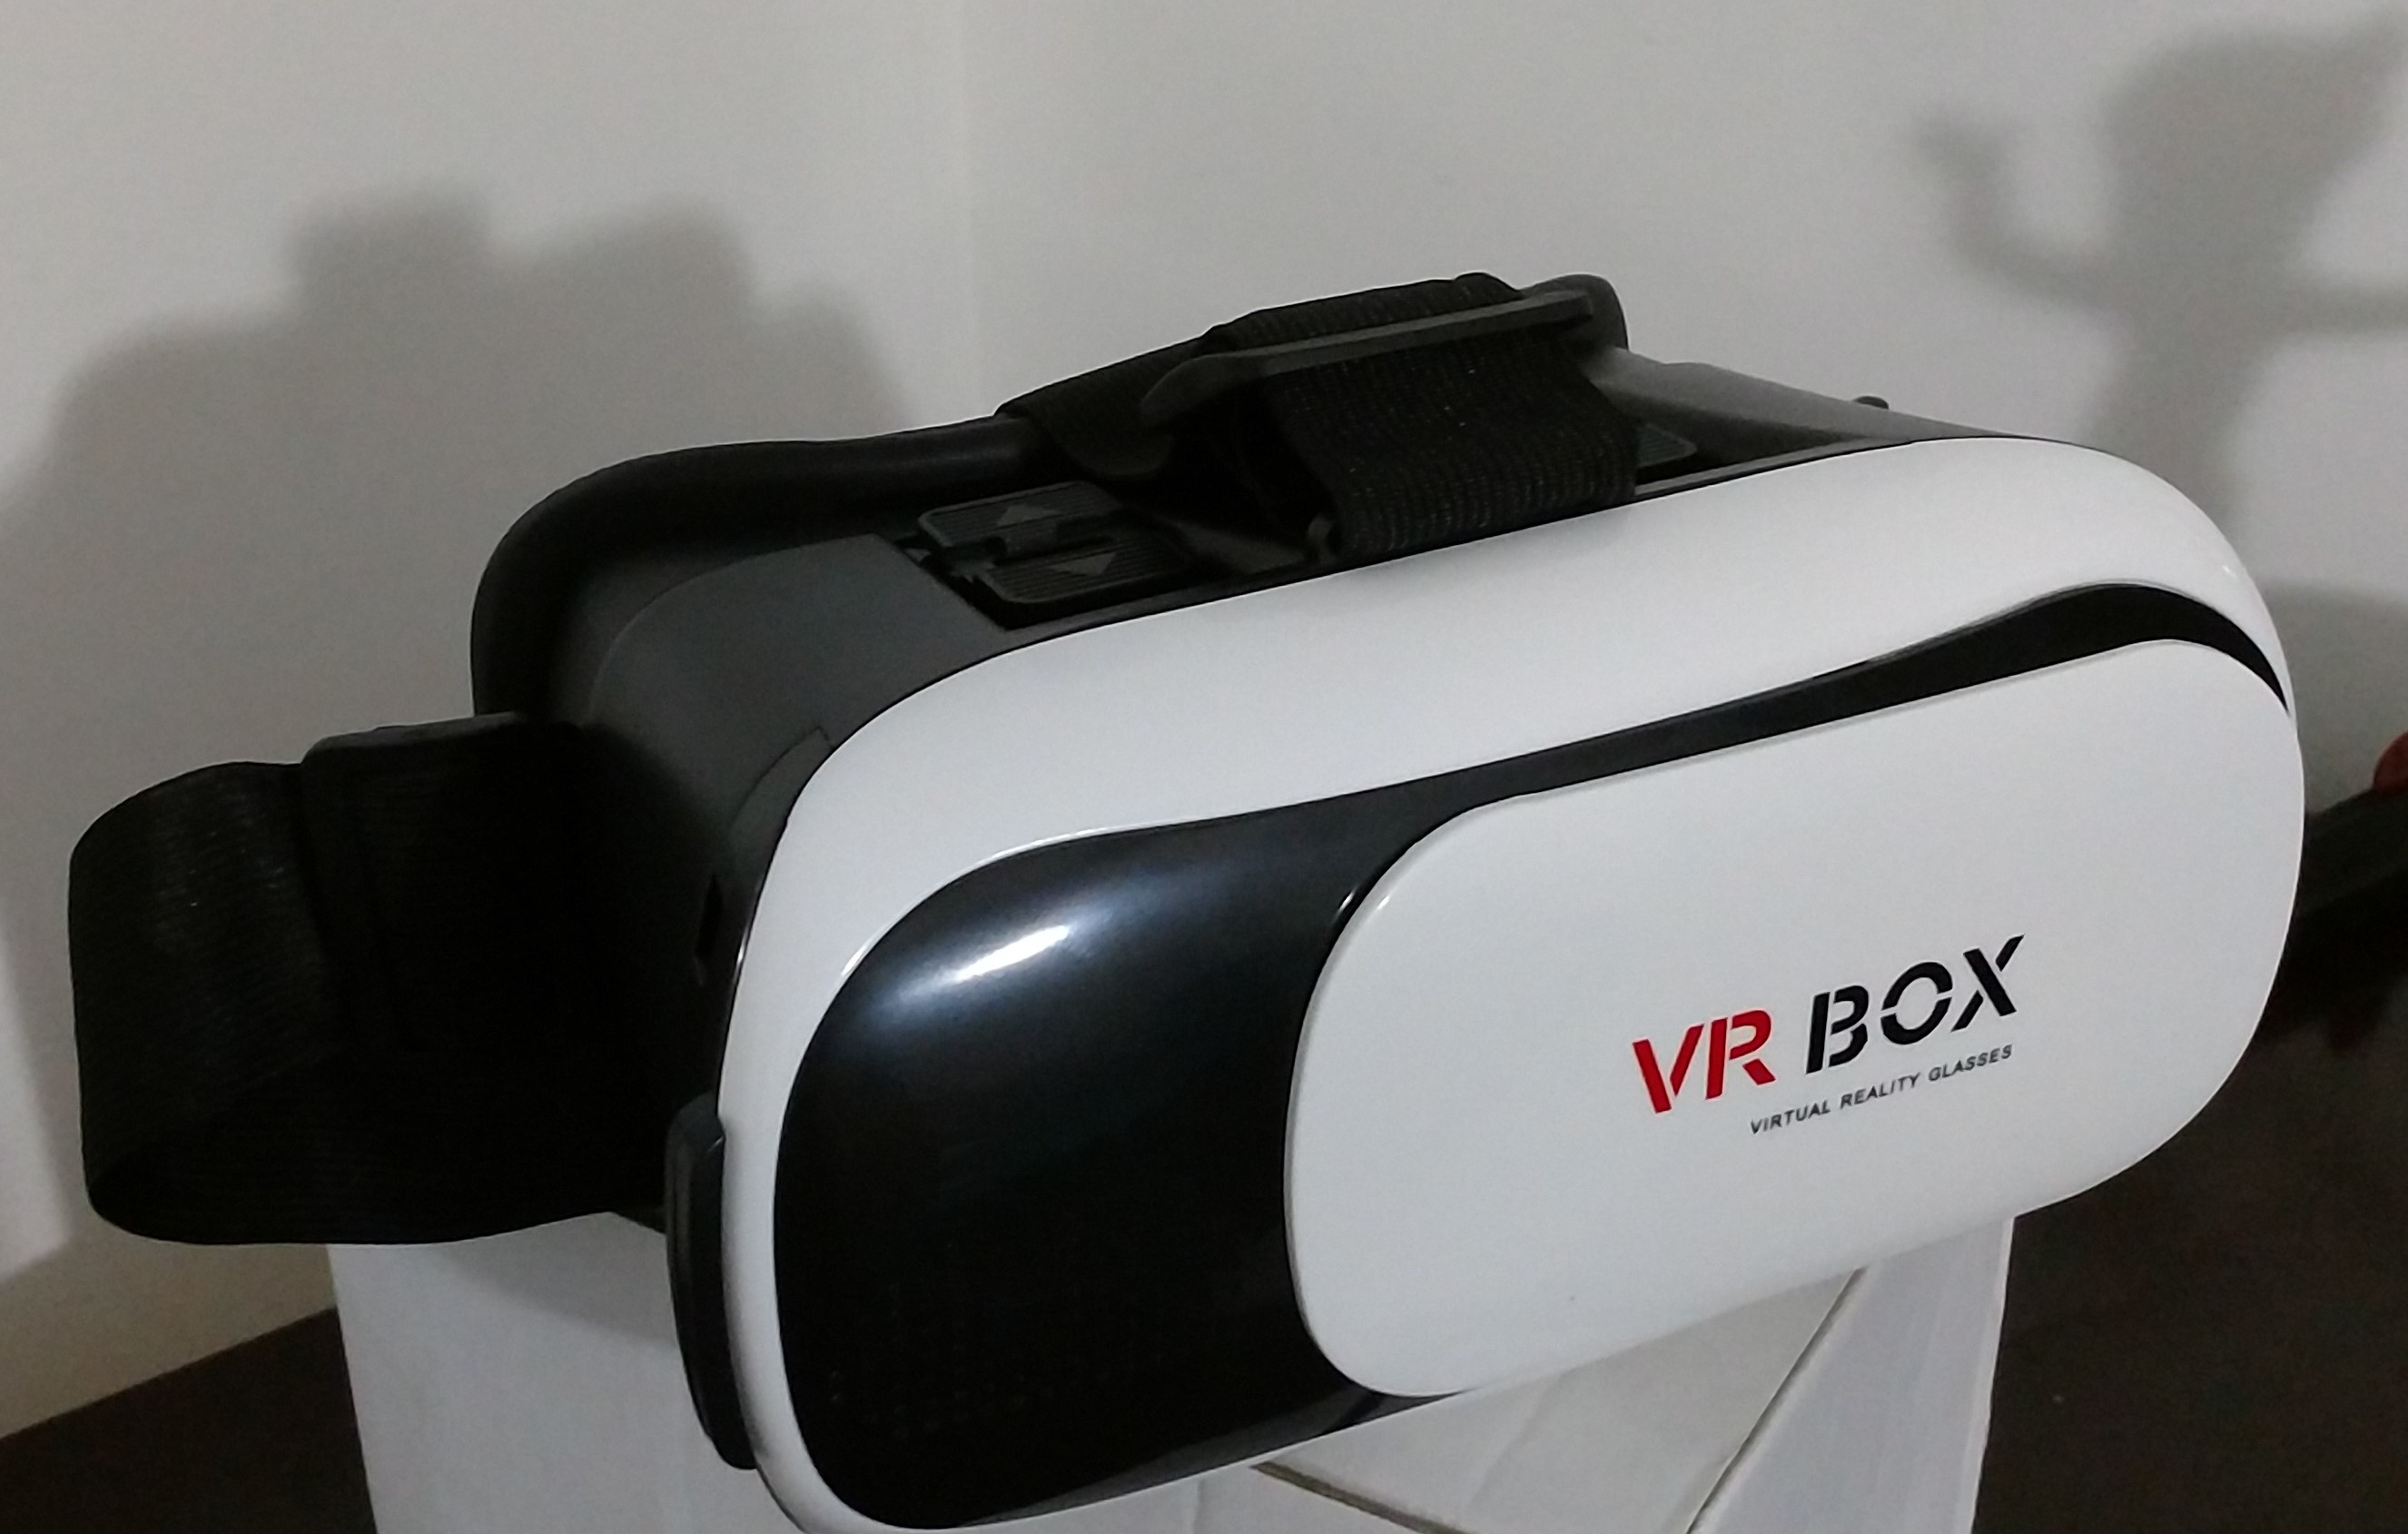
\includegraphics[height=4cm]{Imagens/vrbox.jpg}		
			\label{f.vrbox}
			\legend{\small Fonte: Elaborada pelo autor.}	
		}
	\end{minipage}
	
\end{figure}

Com o Google Cardboard todas as pessoas podem obter uma experiência de imersão em RV de forma simples e barata. É possível montar ou comprar um visualizador e obter a realidade virtual em \textit{smartphones} através de aplicações. \cite{googlecardboard}

O Google Cardboard 2.0 pode ser adquirido em diversos modelos como mostra a Figura ~\ref{f.modelos}. Apesar da primeira versão do Cardboard contar com um modelo para a montagem do visualizador, o modelo da segunda versão ainda não foi disponibilizado pela empresa, apesar de existir modelos de outras fontes.

\begin{figure}[H]
	\caption{\small Google Cardboard V2 Modelos}
	\centering
	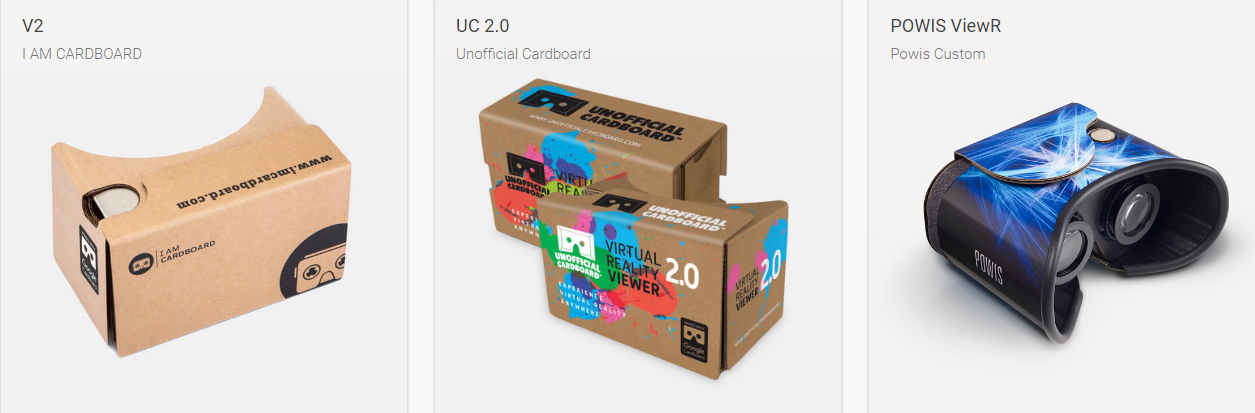
\includegraphics[height=5cm]{Imagens/modelos.png}
	\label{f.modelos}
	\legend{\small Fonte: \citeonline{googlecardboard}.}
\end{figure}

Originalmente, o Google Cardboard não possui suporte para a fixação na cabeça do usuário, ou seja, o usuário terá que segurar o visualizador durante toda a experiência em RV, o que dificulta o uso de controles externos já que os mesmos deverão ser utilizados com somente uma das mãos do usuário. O visualizador comporta \textit{smartphones} com tela de 4.7 até 5.5 polegadas.

O visualizador VR Box vem acompanhado de um controle com comunicação \textit{Bluetooth} que já possui o suporte para cabeça. Diferentemente do Google Cardboard, o VR Box possui um compartimento ajustável para a inserção do \textit{smartphone} (Figura ~\ref{f.extensor}), possibilitando uma melhor fixação de \textit{smartphones} de diversos tamanhos (com telas de 4,7 até 6 polegadas) ao visualizador.

\begin{figure}[H]
	\caption{\small Compartimento para \textit{smartphone}}
	\centering
	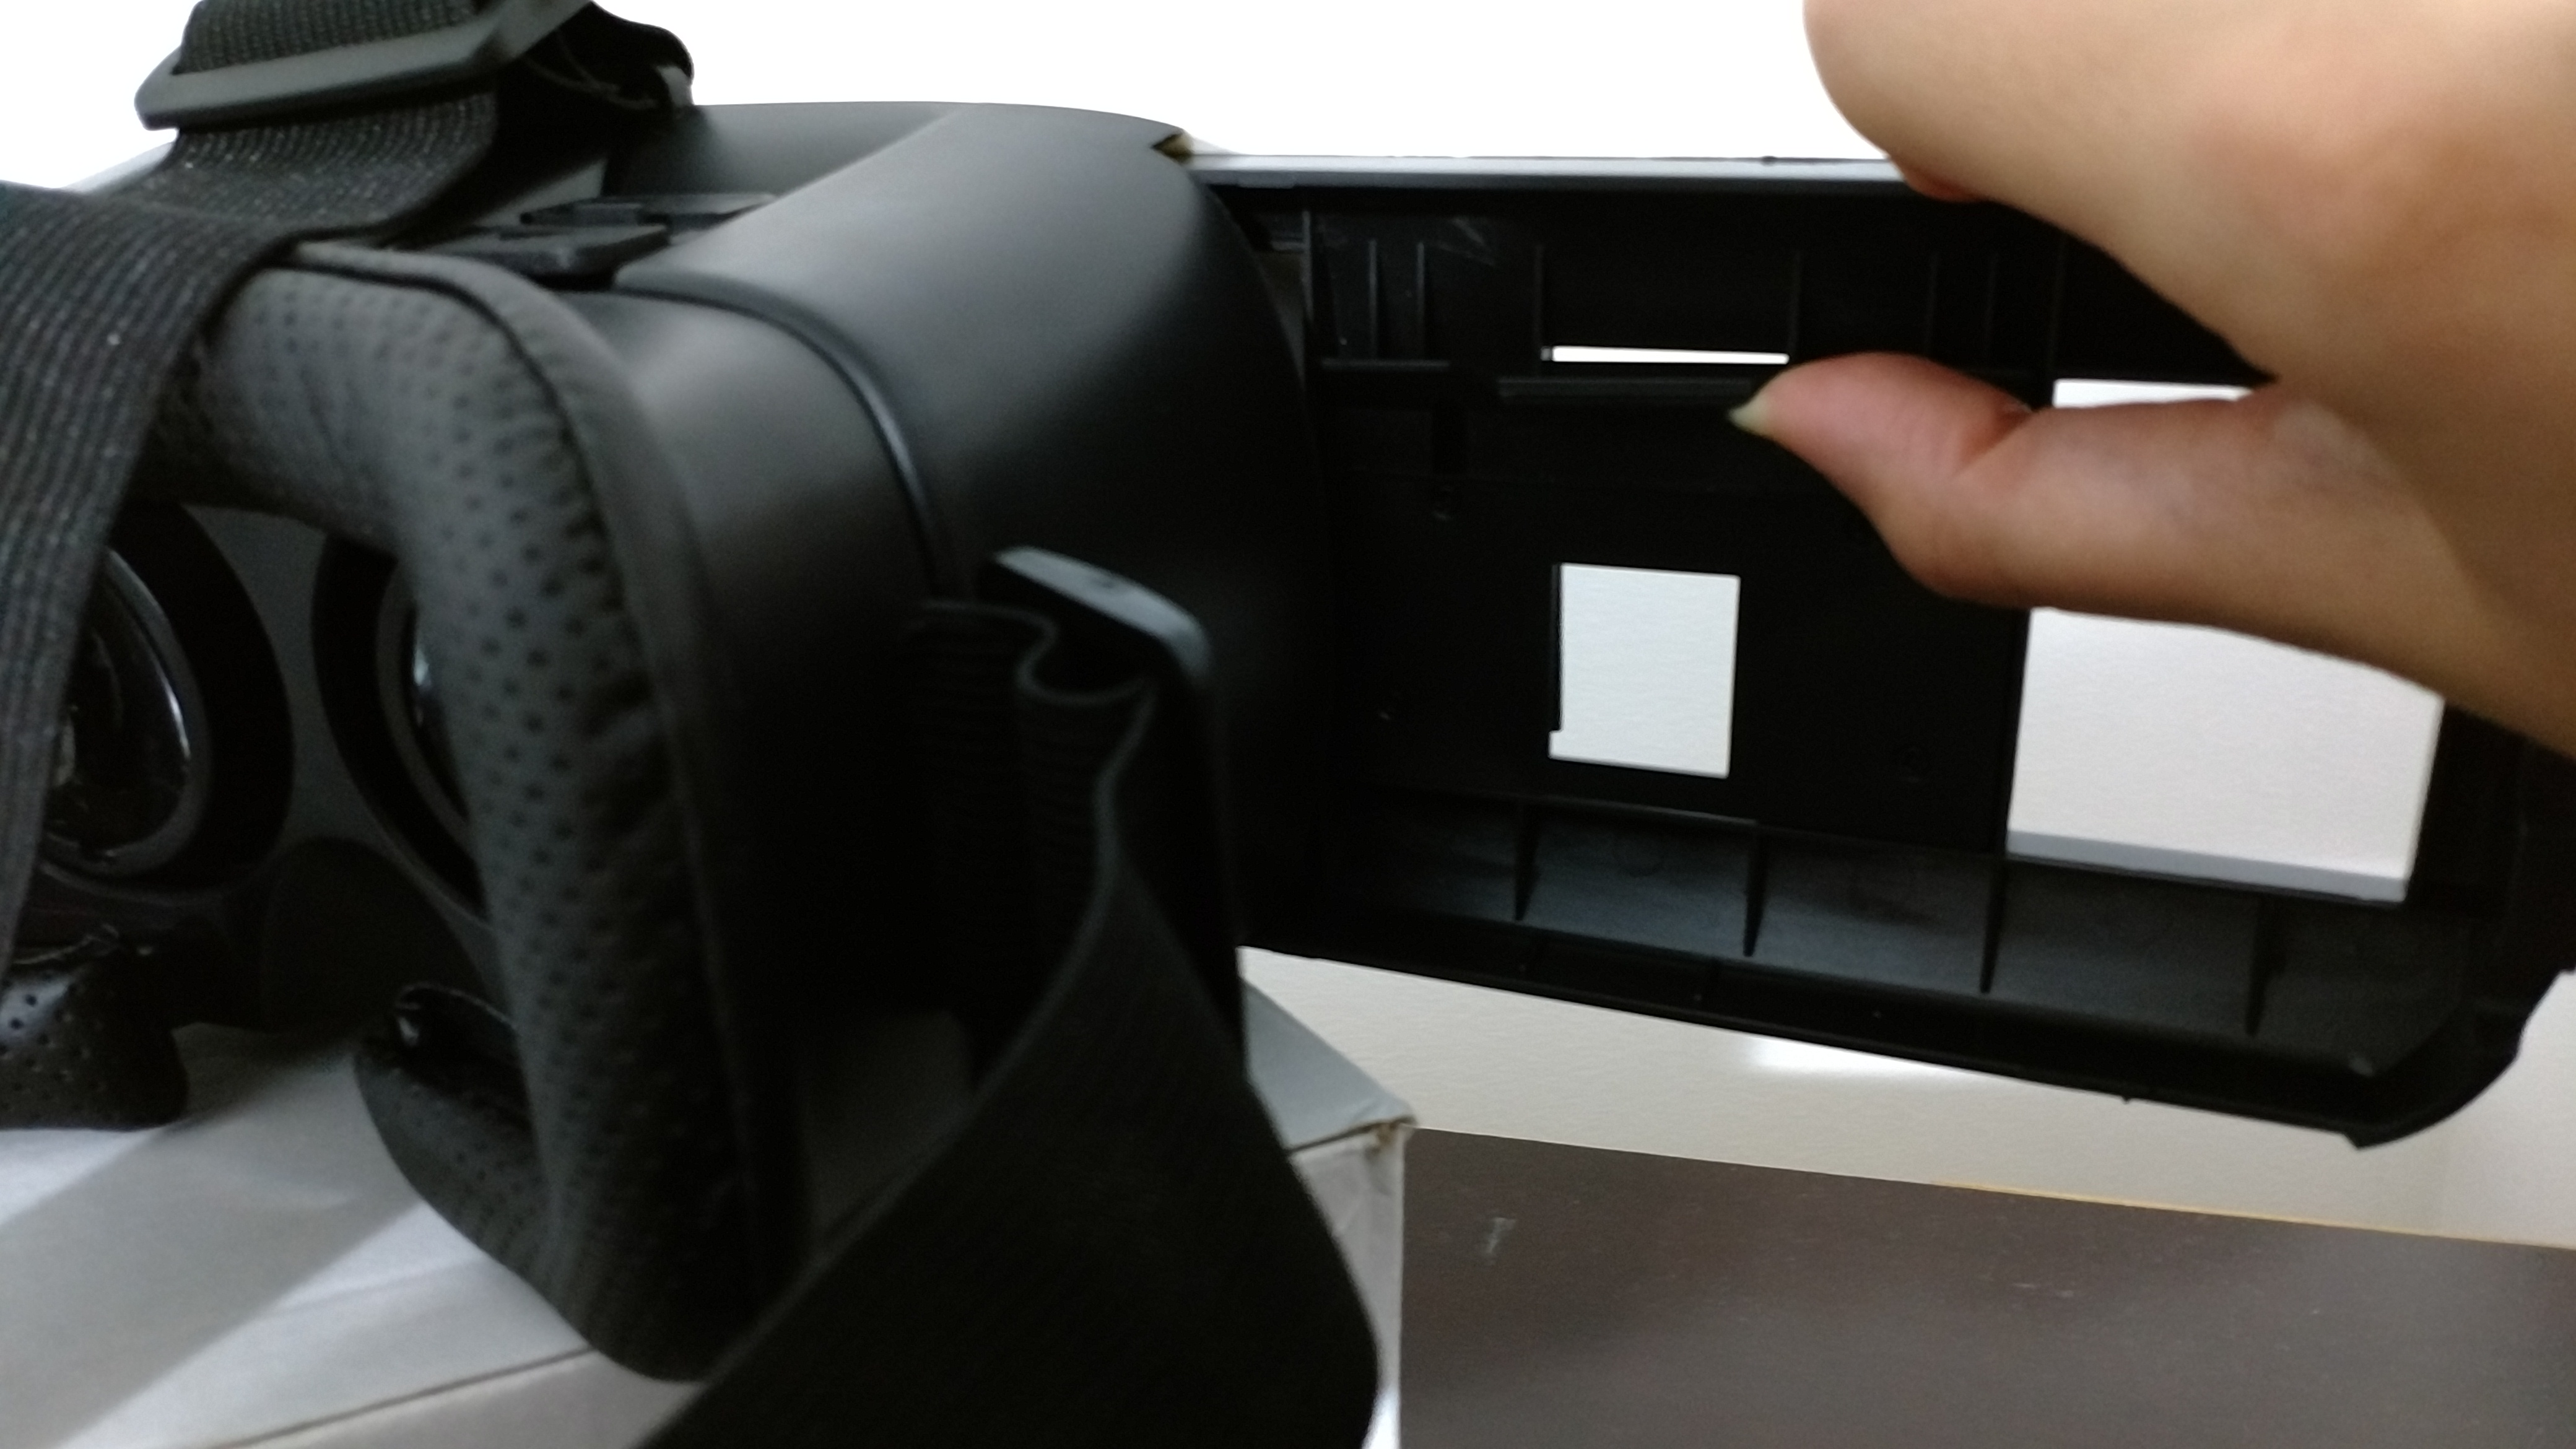
\includegraphics[height=5cm]{Imagens/extensor.jpg}
	\label{f.extensor}
	\legend{\small Fonte: Elaborada pelo autor.}
\end{figure}



\subsection{Dispositivo Móvel}
\label{s.dispositivomovel}

Para se obter uma experiência completa em RV, é necessário que o dispositivo móvel possua giroscópio e acelerômetro. Ao adquirir o Google Cardboard é necessário observar as especificações do visualizador para saber quais tamanhos de telas são suportadas. 

Os testes previstos neste projeto foram realizados em um \textit{smartphone} da Motorola®, modelo Moto X XT1060. As especificações principais deste dispositivo podem ser visualizadas na Tabela ~\ref{t.motox}.

\begin{table}[H]	
	\caption{Especificações Técnicas Moto X} 
	\label{t.motox} 
	\centering
	\begin{tabular}{l|l}
		\textbf{\small Sistema operacional} & {\small Android 5.1 (Lollipop)} \\\hline
		
		\textbf{\small Dimensões} & {\small 129.3 x 65.3 x 10.4 mm (5.09 x 2.57 x 0.41 in)}  \\\hline	
		
		\textbf{\small Peso} & {\small 130 g (4.59 oz)}  \\\hline		 
		
		\textbf{\small Tela} & {\small AMOLED capacitiva touchscreen, 16M cores}  \\\hline  
		
		\textbf{\small Tamanho da tela} & {\small 4,7 polegadas} \\\hline
			
		\textbf{\small Resolução da tela} & {\small 720 x 1280 pixels} \\\hline
		
		\textbf{\small CPU} & {\small Dual-core 1.7 GHz Krait 300} \\\hline
		
		\textbf{\small GPU} & {\small Adreno 320} \\\hline
		
		\textbf{\small Memória} & {\small 16GB} \\\hline
		
		\textbf{\small Bluetooth} & {\small v4.0, A2DP, EDR, LE} \\\hline
		
		\textbf{\small USB} & {\small microUSB v2.0, USB Host} \\\hline	
		
		\textbf{\small Sensores} & {\small Acelerômetro, giroscópio, proximidade, bússola, barômetro, temperatura} \\\hline	
	\end{tabular}
	\legend{\small Fonte: \citeonline{motox}}	
\end{table}

\section{Aplicação ''Vença o Mosquito''}
\label{s.aplicacao}

\subsection{Descrição da Aplicação}
\label{ss.descricao}

Na aplicação desenvolvida, o usuário explora uma área que contém vários objetos. O objetivo do usuário é o de se movimentar no espaço criado por meio de um controle físico, procurando objetos específicos ao redor movimentando a cabeça e executando ações sobre os mesmos.

A fim de contextualizar o usuário no ambiente e definir os objetos que receberão ações, a aplicação trata o combate ao mosquito \textit{Aedes aegypti}, onde o usuário terá que eliminar os focos do mosquito no quintal de uma casa. 

O \citeonline{riodejaneiro} publicou em seu \textit{website} os lugares propícios para a reprodução do mosquito juntamente com as precauções que a população deve tomar para a eliminação do \textit{Aedes aegypti}. Os usuários da aplicação deverão realizar seis das quinze prevenções fornecidas pelo \textit{website} que são:

•	Coloque areia no prato dos vasos de plantas.

•	Mantenha o saco de lixo bem fechado e fora do alcance de animais até o recolhimento pelo serviço de limpeza urbana. Não jogue lixo em terrenos baldios.

•	Troque diariamente a água dos bebedouros de animais e aves e limpe-os com escova ou bucha.

•	Entregue seus pneus velhos ao serviço de limpeza urbana ou guarde-os sem água em local coberto e abrigados da chuva.

•	Guarde as garrafas vazias sempre de cabeça para baixo e de preferência em local coberto.

•	Limpe constantemente as calhas, remova tudo que possa impedir a passagem da água, a laje e a piscina de sua casa.

\subsection{Ações}
\label{ss.acoes}

O usuário conta com cinco ações dentro da aplicação: andar, agachar, selecionar, clicar e abrir o menu. Os caminhos possíveis que o usuário pode percorrer são determinados por objetos que servem como guias dentro da aplicação. Ao clicar nos guias, o usuário irá caminhar até os mesmos, podendo atingir seis posições no cenário como mostra a Figura ~\ref{f.posicoes}.

\begin{figure}[H]
	\caption{\small Posições possíveis na aplicação}
	\centering
	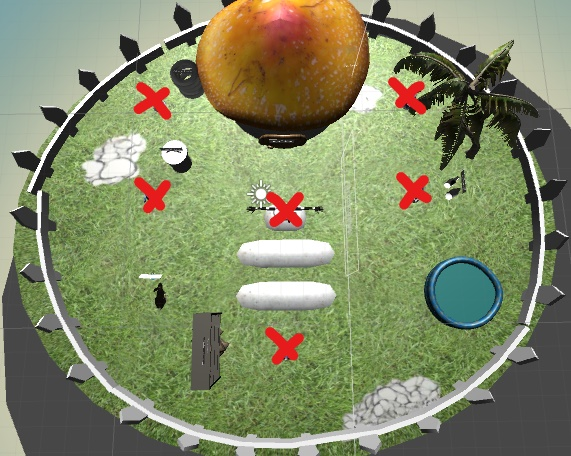
\includegraphics[scale=0.50]{Imagens/posicoes.jpg}
	\label{f.posicoes}
	\legend{\small Fonte: Elaborada pelo autor.}
\end{figure}

Os objetos que poderão sofrer ações possuem um menu que é acionado enquanto o usuário foca o objeto. Este menu mostrará qual ação é permitida para aquele determinado objeto e o usuário poderá executar a ação ao clicar no menu. A Tabela ~\ref{t.acoes} demonstra como cada controle executará as ações citadas acima. 

\begin{table}[H]	
	\caption{Ações dos dispositivos} 
	\label{t.acoes} 
	\centering
	\begin{tabular}{p{2.2cm}|p{2.2cm}|p{2.2cm}|p{2.2cm}|p{2.2cm}|p{2.2cm}}		
		\textbf{\small Dispositivo de controle} & \multicolumn{5}{c}{\textbf{\small Ações}}  \\ \hline \hline
		{} & {\small Andar} & {\small Agachar}  & {\small Selecionar} & {\small Clicar}  & {\small Abrir Menu}\\\hline \hline
		{\small Google Cardboard 2.0} & {\small Selecionar o objeto guia e efetuar o clique} & {\small Manter o botão pressionado} &{\small Olhar para o objeto} & {\small Pressionar e soltar o botão} & {\small Selecionar o botão do menu (localizado na porta da casa) e efetuar o clique}\\\hline		 
		{\small Controle PS2} & {\small Selecionar o objeto guia e efetuar o clique} & {\small Botão O} &{\small Olhar para o objeto} & {\small Botão X} & {\small Botão Select}\\\hline		 
		{\small Controle VRBox} & {\small Selecionar o objeto guia e efetuar o clique} & {\small O menor botão localizado na lateral frontal do controle} &{\small Olhar para o objeto} & {\small O maior botão localizado na lateral frontal do controle} & {\small Botão C}\\\hline  		 
		{\small Teclado} & {\small Selecionar o objeto guia e efetuar o clique} & {\small Botão “Down”} &{\small Olhar para o objeto} & {\small Botão “Space”} & {\small Botão “Escape”} 	\\\hline		
	\end{tabular}
	\legend{\small Fonte: Elaborada pelo autor}	
\end{table}
